
\documentclass[11pt,fleqn]{article} 
\usepackage[margin=0.8in, head=0.8in]{geometry} 
\usepackage{amsmath, amssymb, amsthm}
\usepackage{fancyhdr} 
\usepackage{palatino, url, multicol}
\usepackage{graphicx, pgfplots,xfrac} 
\usepackage[all]{xy}
\usepackage{polynom} 
%\usepackage{pdfsync} %% I don't know why this messes up tabular column widths
\usepackage{enumerate}
\usepackage{framed}
\usepackage{setspace}
\usepackage{array,tikz}

\pgfplotsset{compat=1.6}

\pgfplotsset{soldot/.style={color=black,only marks,mark=*}} \pgfplotsset{holdot/.style={color=black,fill=white,only marks,mark=*}}

\usetikzlibrary{calc}
\tikzstyle{vertex}=[circle, draw, fill=black, inner sep=1pt, minimum size=6pt]


\pagestyle{fancy} 
\lfoot{}
\rfoot{ R6: 3-9 \& 4-1 prep}

\begin{document}
\renewcommand{\headrulewidth}{0pt}
\newcommand{\blank}[1]{\rule{#1}{0.75pt}}
\newcommand{\bc}{\begin{center}}
\newcommand{\ec}{\end{center}}
\renewcommand{\d}{\displaystyle}

\vspace*{-0.7in}

%%%%%%%%%intro page
\begin{center}
  \large
  \sc{Recitation: Week 7}\\ 
\end{center}
 This work sheet has three parts:
 \begin{itemize}
 \item a mini-practice derivative proficiency
 \item a refresher on exponential functions and logarithms
 \item background information for completing the problems from Section 4.1.
 \end{itemize}
  
 
 \begin{center} Mini-Derivative Proficiency \end{center}
You have 10 minutes to write the derivatives of the six functions (three on this page and three on the next). You do not need to simplify. You do need to identify that you are taking the derivative (i.e. write $y'$ or $f'(x)$ or whatever is proper notation.)

 \begin{enumerate}
 \item \large{$g(x)=4x^{\pi}-e^2$}
 \vfill
 \item  \large{$f(\theta)=\theta \tan (2 \theta)$}
 \vfill
 \item  \large{$\displaystyle{y=\frac{-3}{\sqrt{4-x^2}}}$}
 \vfill
 \newpage
 \item \large{$f(x)=\frac{\cos(x)}{x^3 -x}$} (Use the Quotient Rule.)
 \vfill
 \item  \large{$y=2x+\sqrt{3x+\sin(4x)}$}
 \vfill
 \item Find $dy/dx$ for \large{$x^3 y^3=\sin(x+y)$ }
 \vfill
 \end{enumerate}
 \newpage
 \begin{center} Exponential functions and Logarithms \end{center}
 \begin{enumerate}
 \item On the same set of axes, plot the functions below \emph{by plotting at least 4 points on each graph.} $ y=2^x, \quad y=2^{-x}, \quad y=3^{x}$
 \vspace{2in}
 \item Without plotting any points, on the axes above, sketch $y=e^x$ and explain why you made the choice you did.
 \item Explain in simple terms what is meant by the function $y=\log_2 (x).$
 \vfill
 \item Explain in words how to calculate $\log_2(16)$ and $\log_2(\frac{1}{8})$ and how to estimate $\log_2(30).$
 \vfill
 \item Explain how to calculate $\ln (1)$ and $\ln (\frac{1}{e^2}).$ Estimate $\ln(3).$
 \vfill
 \item Explain why $\ln(x^3) = 3 \ln(x).$
 \vfill
 \item (Section 3.9 \#359) Let $P(t)$ denote a population of insects that is increasing a rate of 2 \% per year. If it has an initial population of a thousand insects, Write the exponential function that relates the total population as a function of $t$ and use this expression to determine how large the population is in 10 years.
 \vfill 
 
 \end{enumerate}
 \newpage
 \begin{center} Background for Section 4.1 Problems \end{center}
 \begin{enumerate}
 \item You will need the following formulas. Draw and label a picture for each formula. (Note that at the \emph{bottom} of this page are hints about which formula goes with which problem. Don't look unless you get stuck.)
 	\begin{enumerate}
	\item The Pythagorean Theorem
	\vfill
	\item Sides of Similar Triangles (both right triangles and isosceles triangles)
	\vfill
	\item The Volume and Surface Area of a Sphere of Radius $r.$
	\vfill
	\item The Volume of a Pyramid with a Square Base.
	\vfill
	\item The Volume of a Cone with Base of Radius $r.$
	\vfill
	\end{enumerate}
\item Assume that the length of side labeled $a$ in the picture below is changing over time. What would be a good symbol to represent ``the change in $a$ with respect to time"? What can you say about this rate of change if side $a$ is getting shorter? longer? not changing in length?\\
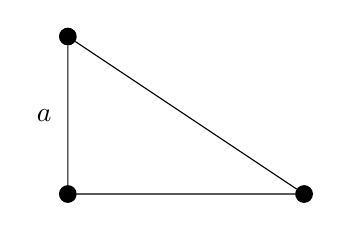
\begin{tikzpicture}
\node[vertex] (a) at (0,0){};\node[vertex] (b) at (0,2){};\node[vertex] (c) at (3,0){};
\draw (a) -- (b) -- (c) -- (a);
\node at (-.3,1){$a$};
\end{tikzpicture}
 \end{enumerate}
 
 (a) \#5,7,9 (b) \#11,12,31 (c) \# 19 (d) \# 31 (e) \# 35
\end{document}

